\documentclass{article}

\usepackage{pdfpages}
\usepackage{graphicx}
\usepackage{longtable}
%\usepackage[export]{adjustbox}
%\usepackage{tabu}
\usepackage{xcolor,colortbl}
\usepackage{caption}
\usepackage{subcaption}
\usepackage{float}

\usepackage[margin=0.65in]{geometry}

\begin{document}

\vspace*{3ex}
\begin{flushright}
{\large 10 November 2015}
\end{flushright}

\vskip20ex
\hskip3cm

\begin{center}


\begin{figure}[H]
\centering
\begin{subfigure}{.5\textwidth}
  \centering
  
\includegraphics[width=.9\linewidth]{images/mini.png}
\end{subfigure}%
\begin{subfigure}{.5\textwidth}
  \centering
  
\includegraphics[width=.9\linewidth]{images/pw.jpg}
\end{subfigure}
\end{figure}




\Large {\bf
	Bachelor Thesis \\
	Finite Automata for Pattern Recognition
}

\Large {\bf 
	Technical Project
}
\end{center}
\vskip2ex


\vskip25ex

\begin{flushleft}
{\large Bartlomiej Dybisz \\
Jakub Ciecierski

}
\end{flushleft}

\newpage
\tableofcontents
\newpage

%------------------------------------------------------------------------------

\section*{Document metric}

\begin{center}


\begin{table}[h]
\hspace*{-1.1cm}
\large
\begin{tabular}{|
>{\columncolor[HTML]{C0C0C0}}l |l|l|l|l|l|}
\hline
\multicolumn{6}{|l|}{\cellcolor[HTML]{C0C0C0}Document metric}                                                                                                                                         \\ \hline
Project:       & \multicolumn{2}{l|}{Finite automata for pattern recognition} & 
\cellcolor[HTML]{C0C0C0}Company: & \multicolumn{2}{l|}{WUT}                                               \\ \hline
Name:          & \multicolumn{5}{l|}{Technical Project}                                                                                                                                       \\ \hline
Topics:        & \multicolumn{5}{l|}{Architecture and algorithms defining the project}                                                                                                                                       \\ \hline
Author:        & \multicolumn{5}{l|}{Jakub Ciecierski, Bartlomiej Dybisz}                                                                                                                                                \\ \hline
File:          & \multicolumn{5}{l|}{technical\_project.pdf}                                                                                                                                      \\ \hline
Version no:    & 0.1                                                                      & \cellcolor[HTML]{C0C0C0}Status:  & Under development & \cellcolor[HTML]{C0C0C0}Opening date: & 2015-10-27 \\ \hline
Summary:       & \multicolumn{5}{l|}{Technical side of research on pattern recognition by finite automata}                                                                                                           \\ \hline
Authorized by: & \begin{tabular}[c]{@{}l@{}}Wladyslaw Homenda\end{tabular} & \multicolumn{3}{l|}{\cellcolor[HTML]{C0C0C0}Last modification date:}                         & 2015-11-10 \\ \hline
\end{tabular}
\end{table}

\end{center}



\section*{History of changes}

\begin{center}


\begin{table}[h]
\hspace*{-1.0cm}
\large
\begin{tabular}{|l|l|l|l|}
\hline
\multicolumn{4}{|l|}{\cellcolor[HTML]{C0C0C0}History of Changes} \\ \hline
Version         & Date         & Who        & Description        \\ \hline

0.1         
& 2015-11-10
& Jakub Ciecierski, Bartlomiej Dybisz
& Definition of the main purpose of the document       \\ \hline
\end{tabular}
\end{table}

\end{center}


%---------------------------------------------------------------

\section*{Schedule}

\begin{center}


\begin{table}[h]

\large
\begin{tabular}{|l|l|l|}
\hline
\multicolumn{3}{|l|}{\cellcolor[HTML]{C0C0C0}Schedule} \\ \hline
Date         & Note        & Planned Progress          \\ \hline
\hline

27.10.2015   & Lab1    & Presentation of Business Analysis   \\ \hline
03.11.2015   &    & Additional changes of Business Analysis   \\ \hline
7-9.11.2015   &     & First drafts of UML of particular modules   \\ \hline
14-16.11.2015   &     & Requirements analysis, design of algorithms and further UML development \\ \hline
17.11.2015   &  Lab2   & Presentation of Technical Analysis   \\ \hline
20-22.11.2015   &     & Implementation of mudules needed for testing and basic GUI   \\ \hline
31.11.2015   & Lab3    & Presentation of results of tests on synthetic and semi-synthetic data  \\ \hline
4-6.12.2015   &     & GUI and console application development  \\ \hline
15.12.2015   & Lab4    & Final GUI  \\ \hline
-------  & -------    & Work depends on acquired results  \\ \hline
08.01.2015  & Lab5    & Complete system presentation  \\ \hline
\end{tabular}
\end{table}

\end{center}


%---------------------------------------------------------------
\newpage




%---------------------------------------------------------------
\section{Production Model}
{\bf Waterfall} model is a model which was developed for software development; that is to create software. It is called as such because the model develops systematically from one phase to other in a downward fashion, like a waterfall.

{\color{red} NICE DECRIPTION LOL}

\begin{center}

	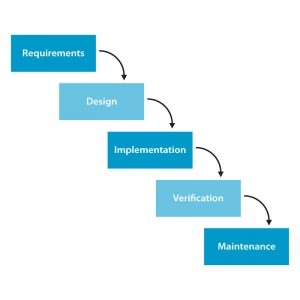
\includegraphics[width=80mm]{images/waterfall_model.jpg}

\end{center}


%---------------------------------------------------------------
\section{Technology}

%---- JC ----%


%---- BD ----%



\newpage


%---------------------------------------------------------------
\section{Algorithms}

%---- JC ----%


%---- BD ----%


%---------------------------------------------------------------
%---------------------------------------------------------------
\subsubsection{Examples}
% Examples of algorithms, if any.

%---- JC ----%


%---- BD ----%

%---------------------------------------------------------------
\section{Data structures}

%---- JC ----%


%---- BD ----%

%---------------------------------------------------------------
\section{Modules}
	
%---- JC ----%


%---- BD ----%

%---------------------------------------------------------------
\section{Modelling}

%---- JC ----%


%---- BD ----%


\end{document}


